%File: anonymous-submission-latex-2026.tex
\documentclass[letterpaper]{article} % DO NOT CHANGE THIS
\usepackage[submission]{aaai2026}  % DO NOT CHANGE THIS
\usepackage{times}  % DO NOT CHANGE THIS
\usepackage{helvet}  % DO NOT CHANGE THIS
\usepackage{courier}  % DO NOT CHANGE THIS
\usepackage[hyphens]{url}  % DO NOT CHANGE THIS
\usepackage{graphicx} % DO NOT CHANGE THIS
\urlstyle{rm} % DO NOT CHANGE THIS
\def\UrlFont{\rm}  % DO NOT CHANGE THIS
\usepackage{natbib}  % DO NOT CHANGE THIS AND DO NOT ADD ANY OPTIONS TO IT
\usepackage{caption} % DO NOT CHANGE THIS AND DO NOT ADD ANY OPTIONS TO IT
\frenchspacing  % DO NOT CHANGE THIS
\setlength{\pdfpagewidth}{8.5in} % DO NOT CHANGE THIS
\setlength{\pdfpageheight}{11in} % DO NOT CHANGE THIS
%
% These are recommended to typeset algorithms but not required. See the subsubsection on algorithms. Remove them if you don't have algorithms in your paper.
\usepackage{algorithm}
\usepackage{algorithmic}
\usepackage{booktabs}
\usepackage{makecell}
\usepackage{multirow}
\usepackage{amssymb} 
\usepackage{amsmath}
\usepackage{xcolor}     % \textcolor{red}
%
% These are are recommended to typeset listings but not required. See the subsubsection on listing. Remove this block if you don't have listings in your paper.
\usepackage{newfloat}
\usepackage{listings}
\DeclareCaptionStyle{ruled}{labelfont=normalfont,labelsep=colon,strut=off} % DO NOT CHANGE THIS
\lstset{%
	basicstyle={\footnotesize\ttfamily},% footnotesize acceptable for monospace
	numbers=left,numberstyle=\footnotesize,xleftmargin=2em,% show line numbers, remove this entire line if you don't want the numbers.
	aboveskip=0pt,belowskip=0pt,%
	showstringspaces=false,tabsize=2,breaklines=true}
\floatstyle{ruled}
\newfloat{listing}{tb}{lst}{}
\floatname{listing}{Listing}
%
% Keep the \pdfinfo as shown here. There's no need
% for you to add the /Title and /Author tags.
\pdfinfo{
/TemplateVersion (2026.1)
}

% DISALLOWED PACKAGES
% \usepackage{authblk} -- This package is specifically forbidden
% \usepackage{balance} -- This package is specifically forbidden
% \usepackage{color (if used in text)
% \usepackage{CJK} -- This package is specifically forbidden
% \usepackage{float} -- This package is specifically forbidden
% \usepackage{flushend} -- This package is specifically forbidden
% \usepackage{fontenc} -- This package is specifically forbidden
% \usepackage{fullpage} -- This package is specifically forbidden
% \usepackage{geometry} -- This package is specifically forbidden
% \usepackage{grffile} -- This package is specifically forbidden
% \usepackage{hyperref} -- This package is specifically forbidden
% \usepackage{navigator} -- This package is specifically forbidden
% (or any other package that embeds links such as navigator or hyperref)
% \indentfirst} -- This package is specifically forbidden
% \layout} -- This package is specifically forbidden
% \multicol} -- This package is specifically forbidden
% \nameref} -- This package is specifically forbidden
% \usepackage{savetrees} -- This package is specifically forbidden
% \usepackage{setspace} -- This package is specifically forbidden
% \usepackage{stfloats} -- This package is specifically forbidden
% \usepackage{tabu} -- This package is specifically forbidden
% \usepackage{titlesec} -- This package is specifically forbidden
% \usepackage{tocbibind} -- This package is specifically forbidden
% \usepackage{ulem} -- This package is specifically forbidden
% \usepackage{wrapfig} -- This package is specifically forbidden
% DISALLOWED COMMANDS
% \nocopyright -- Your paper will not be published if you use this command
% \addtolength -- This command may not be used
% \balance -- This command may not be used
% \baselinestretch -- Your paper will not be published if you use this command
% \clearpage -- No page breaks of any kind may be used for the final version of your paper
% \columnsep -- This command may not be used
% \newpage -- No page breaks of any kind may be used for the final version of your paper
% \pagebreak -- No page breaks of any kind may be used for the final version of your paperr
% \pagestyle -- This command may not be used
% \tiny -- This is not an acceptable font size.
% \vspace{- -- No negative value may be used in proximity of a caption, figure, table, section, subsection, subsubsection, or reference
% \vskip{- -- No negative value may be used to alter spacing above or below a caption, figure, table, section, subsection, subsubsection, or reference

\setcounter{secnumdepth}{0} %May be changed to 1 or 2 if section numbers are desired.

% The file aaai2026.sty is the style file for AAAI Press
% proceedings, working notes, and technical reports.
%

% Title

% Your title must be in mixed case, not sentence case.
% That means all verbs (including short verbs like be, is, using,and go),
% nouns, adverbs, adjectives should be capitalized, including both words in hyphenated terms, while
% articles, conjunctions, and prepositions are lower case unless they
% directly follow a colon or long dash
\title{AAAI Press Anonymous Submission\\Instructions for Authors Using \LaTeX{}}
\author{
    %Authors
    % All authors must be in the same font size and format.
    Written by AAAI Press Staff\textsuperscript{\rm 1}\thanks{With help from the AAAI Publications Committee.}\\
    AAAI Style Contributions by Pater Patel Schneider,
    Sunil Issar,\\
    J. Scott Penberthy,
    George Ferguson,
    Hans Guesgen,
    Francisco Cruz\equalcontrib,
    Marc Pujol-Gonzalez\equalcontrib
}
\affiliations{
    %Afiliations
    \textsuperscript{\rm 1}Association for the Advancement of Artificial Intelligence\\
    % If you have multiple authors and multiple affiliations
    % use superscripts in text and roman font to identify them.
    % For example,

    % Sunil Issar\textsuperscript{\rm 2},
    % J. Scott Penberthy\textsuperscript{\rm 3},
    % George Ferguson\textsuperscript{\rm 4},
    % Hans Guesgen\textsuperscript{\rm 5}
    % Note that the comma should be placed after the superscript

    1101 Pennsylvania Ave, NW Suite 300\\
    Washington, DC 20004 USA\\
    % email address must be in roman text type, not monospace or sans serif
    proceedings-questions@aaai.org
%
% See more examples next
}

%Example, Single Author, ->> remove \iffalse,\fi and place them surrounding AAAI title to use it
\iffalse
\title{My Publication Title --- Single Author}
\author {
    Author Name
}
\affiliations{
    Affiliation\\
    Affiliation Line 2\\
    name@example.com
}
\fi

\iffalse
%Example, Multiple Authors, ->> remove \iffalse,\fi and place them surrounding AAAI title to use it
\title{My Publication Title --- Multiple Authors}
\author {
    % Authors
    First Author Name\textsuperscript{\rm 1},
    Second Author Name\textsuperscript{\rm 2},
    Third Author Name\textsuperscript{\rm 1}
}
\affiliations {
    % Affiliations
    \textsuperscript{\rm 1}Affiliation 1\\
    \textsuperscript{\rm 2}Affiliation 2\\
    firstAuthor@affiliation1.com, secondAuthor@affilation2.com, thirdAuthor@affiliation1.com
}
\fi


% REMOVE THIS: bibentry
% This is only needed to show inline citations in the guidelines document. You should not need it and can safely delete it.
\usepackage{bibentry}
% END REMOVE bibentry

\begin{document}

\maketitle

\begin{abstract}
AAAI creates proceedings, working notes, and technical reports directly from electronic source furnished by the authors. To ensure that all papers in the publication have a uniform appearance, authors must adhere to the following instructions.
\end{abstract}

% Uncomment the following to link to your code, datasets, an extended version or similar.
% You must keep this block between (not within) the abstract and the main body of the paper.
% \begin{links}
%     \link{Code}{https://aaai.org/example/code}
%     \link{Datasets}{https://aaai.org/example/datasets}
%     \link{Extended version}{https://aaai.org/example/extended-version}
% \end{links}

\section{Introduction}

Predicting drug-drug interactions (DDIs) is important for safe medication use and drug development, and unanticipated DDIs are an important source of preventable hospitalizations and adverse events~\cite{ddi-burden}. 
%
Computational methods have become an established tool for large-scale DDI screening~\cite{ddi-review}.
%
The most demanding setting is the cold-start regime, in which a test pair involves drugs not observed during training, and weak performance on these emerging drugs is a recognized limitation of existing methods~\cite{ddi-difficult}.
%
The strictest form of this setting, in which both drugs of a test pair are unseen, is addressed by graph-based DDI methods that fall into three categories according to the structure they reason over, namely node-based~\cite{Method-RGCN}, path-based~\cite{Method-Emergnn}, and subgraph-based~\cite{Method-Knowddi} methods.
%
We use a rank-truncation analysis to examine the transferability of representative models across these three categories for cold-start setting, as shown in Figure~\ref{fig:intro}. 
%
The transferable component, that is, the information usable for cold-start prediction, is found to be low-rank and to occupy only a low-dimensional subspace. 
%
By contrast, under the warm-start protocol, which uses the same test pairs but allows the two drugs to be seen during training, the rank-truncated AUC-ROC continues to increase into the high-rank region.
%
Across all three models, this low-rank region extends up to the rank at which each first attains 92\% of its full-rank performance.

\begin{figure}[t]
  \centering
  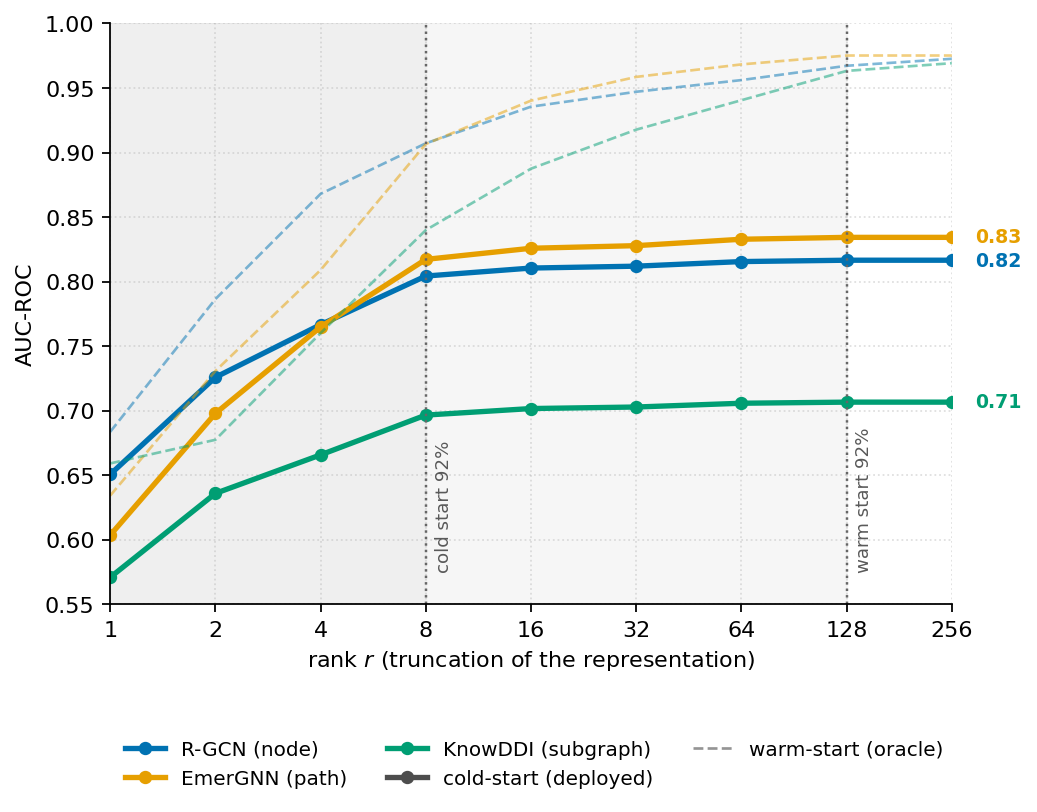
\includegraphics[width=0.9\columnwidth]{Figures/Fig1-intro.png}
  \caption{On the multi-class task ($K{=}79$), the representation learned by three models spanning node, path, and subgraph-based architecture (R-GCN, EmerGNN, KnowDDI) is truncated to rank $r$ and re-evaluated by AUC-ROC. Solid lines denote cold-start (both drugs unseen), and dashed lines denote warm-start (both seen).}
  \label{fig:intro}
\end{figure}

This low-rank structure is empirically observed under cold-start training without any imposed constraint, although its presence is unsurprising because DDIs are driven by a limited set of mediating biological entities (MBEs), such as enzymes, transporters, targets, and systemic effects~\cite{Stockley-book-2018}, to which the transferable signal appears to be tied.
%
However, for such low-rank structure, studies of generalization and invariance indicate that unconstrained training tends to allocate capacity to dominant, high-variance directions, whereas predictive invariant directions need not align with these top-variance directions~\cite{ISR-ICML-2022}.
%
With respect to DDI prediction, this suggests that a model may fit the mechanisms that dominate among seen drugs, even though those mechanisms need not govern unseen drugs, which impairs transfer and can compromise performance on certain mechanism classes.
%
In other words, low rank alone does not determine which directions span the usable subspace, nor does it ensure that the transferable subspace aligns with the biological mechanisms that determine DDIs.
%

This motivates aligning the limited low-rank capacity with the DDI-determining biological mediating entities encoded by the knowledge-graph structure and clarifying how misalignment of the low-rank subspace affects cold-start generalization.
%
More specifically, we propose a low-rank semantic adapter, named \textsc{DDI-LoRA}, inspired by the low-rank adaptation (LoRA)~\cite{Method-Lora-ICLR-2022} originally developed for LLMs.
%
Such adapters commonly serve as auxiliary components that complement a backbone model by providing structural inductive bias or semantic information~\cite{Method-Adapter-ICML-2019}.
%
In our design, \textsc{DDI-LoRA} supplies the frozen backbone with a low-rank correction oriented toward biological semantics.
%
The design is inherently compatible with cold-start prediction, can be incorporated in a unified manner into different graph-based DDI models, and can also serve as a standalone predictor once the base representation of the backbone is removed.
%
The central idea is to treat a drug pair only as a selector over the MBEs in the KG, thereby shifting the modeling target from drug to MBE representations.
%
\textsc{DDI-LoRA} is built from two components, a typed prototype basis $M_B$ and an active-mediator selector $M_A$. The basis $M_B$ holds a small set of prototypes for each mediator type, shared across all drug pairs and independent of any specific drug.
%
The selector $M_A$ activates, for each drug pair, only the prototypes of the shared mediators of the two drugs, the entities that lie within the multi-hop neighborhoods of both drugs in the knowledge graph.
%
With this design, the limited low-rank capacity is further directed toward the biological entities rather than the dominant topological patterns that unconstrained training tends to follow, so that \textsc{DDI-LoRA} steers the model toward the biological mechanisms underlying DDIs. 
%

\textbf{Specific contributions of this paper are as follows:}
\begin{itemize}
    \item A rank-truncation analysis shows that, under cold-start, the transferable DDI signal learned by different backbones is intrinsically low-rank, yet its orientation need not align with the mechanisms governing DDIs.
    
    \item \textsc{DDI-LoRA} is proposed, a parameter-efficient low-rank semantic adapter that orients the limited capacity toward KG-derived biological prototypes and is cold-start friendly by construction.
    
    \item Empirical analysis attributes the gains of \textsc{DDI-LoRA} to biological semantic orientation rather than confounding factors, offering a lightweight solution and a new perspective for cold-start prediction.
\end{itemize}

\section{Related Work}

\subsection{Graph-Based DDI Prediction Under Cold Start}

Graph-based methods have become the dominant paradigm for DDI prediction, since drug interactions are naturally represented as edges between drug nodes and biomedical knowledge graphs already encode rich relational priors over these interactions~\cite{BKG-Hetionet,BKG-Primekg}.
%
These methods can be organized by the structure over which a drug pair is scored, progressing from node to path to subgraph-based prediction. 
%
At the node level, DDKG~\cite{Method-DDKG} encodes each drug from its knowledge-graph attributes and neighborhood and scores a pair from the two drugs represented independently, and KGNN~\cite{Method-KGNN} likewise aggregates each drug's local neighborhood through a graph neural network.
%
Beyond independent encoding, K-Paths~\cite{Method-K_paths} predicts over the multi-hop paths connecting the two drugs to produce interpretable interaction evidence. 
%
Richer still, SumGNN~\cite{Method-Sumgnn} summarizes an enclosing k-hop subgraph with attention and KnowDDI~\cite{Method-Knowddi} learns a knowledge subgraph for each drug pair, both capturing pair-level evidence at a higher computational cost. 
%
Across this progression, accuracy improves by widening the scope of graph modeling, yet these methods remain centered on warm-start settings in which both drugs are seen during training.
%

By contrast, cold-start remains difficult because a test drug is unseen during training, yet this setting is central for emerging drugs. 
%
Existing approaches reduce the reliance on observed drug identity in two ways. Some derive representations from intrinsic features such as molecular substructure, as in SSI-DDI~\cite{Method-SSI_DDI} and HDN-DDI~\cite{Method-HDN_DDI}, so that a drug never seen during training can still be encoded.
%
Others reason inductively over knowledge-graph neighborhoods, as in EmerGNN~\cite{Method-Emergnn}, so that an emerging drug is reached through its relational context rather than through a learned identity. 
%
Nonetheless, most of these methods focus on how a representation is formed for an unseen drug, while neglecting which biological mechanisms of interaction remain transferable when both endpoints are unseen. 
%
In comparison, this work characterizes the transferable signal as intrinsically low-rank and orients this limited capacity toward the biological mediators that determine DDIs, which is essential for reliable cold-start prediction.


\subsection{Inductive Prediction and Low-Rank Transfer}

\textbf{Inductive relational prediction.} 
Cold-start DDI prediction requires scoring pairs of drugs never observed during training, which rules out any parameter tied to a specific drug's identity.
%
This requirement is the premise of inductive knowledge-graph link prediction, which predicts a relation from the relational context around the two endpoints rather than from learned entity identities.
%
GraIL~\cite{GRAIL-PMLR-2020} scores a candidate relation from the enclosing subgraph using distance-based structural roles, while NBFNet~\cite{NBF-NIPS-2021} scores an entity pair by aggregating messages over the connecting paths, both without per-entity embeddings and both operating when training and test entities are disjoint. 
%
This establishes that pairwise prediction is feasible when both endpoints are unseen, yet it remains open whether, in DDI, the transferable subspace is confined to the few directions determined by the governing biological mechanisms.


\textbf{Low-rank in transfer and adaptation.} 
Currently, two lines of work connect low-rank to transfer and domain-generalization.
%
The first observes that the signal surviving a distribution shift in a low-rank subspace~\cite{LTS-ICDM-2012,DEEPDG-ITIP-2017,ISR-ICML-2022}, attributing this low rank to cross-domain heterogeneity, in which only a small part is shared across domains.
%
The second treats low rank as the intrinsic compressibility of adaptation, showing that strong solutions lie within a random low-dimensional subspace~\cite{INTRINSICDIM-ICLR-2018} and that a model can be adapted by optimizing a low-rank update with few degrees of freedom~\cite{Lora-ICLR-2022}.
%
Within DDI, a representative family carries a similar idea through tensor or matrix factorization, placing low-rank structure on the observed interaction tensor or on per-drug latent factors~\cite{Method-Decagon,Method-CTF_ddi}, while it still reaches new drugs through a drug's similarity to known drugs~\cite{Method-TMFUF}, and it does not map that similarity onto an interpretable biological subspace.
%
The present work differs from all of these. It operates within a single DDI domain, so the low rank here does not stem from cross-domain heterogeneity but from the limited set of biological mediators that determine DDIs. 
%
As for the second line, it adopts the frozen-base and low-rank-update form, although this low rank is not chosen for parameter efficiency but, again, follows from the limited number of these mediators.
%
Lastly, unlike the factorization family, which as noted does not map its latent factors onto a concrete interpretable subspace, the adapter here directs its low-rank capacity onto the typed biological mediators shared by the two drugs.
%
These observations recast cold-start DDI as not primarily a problem of model capacity or of learning better unseen-drug representations, because the transferable interaction signal already resides in a small mediator-defined subspace and the core task is to orient a low-rank correction toward it.
%
Our proposed method actively aligns its directions with specific biological mediators, which directly embodies this view.

\section{Preliminaries}
\subsection{Knowledge Graph and DDI}

\textbf{Knowledge graph.} 
Prediction is performed on a biomedical knowledge graph $G=(V,R,E)$, where $V$ denotes the entity set, $R$ the relation set, and $E$ the set of typed edges, with $E\subseteq V\times R\times V$. 
%
Drug nodes constitute a subset $D\subseteq V$, and non-drug entities such as proteins, side effects, and pathways constitute $V\setminus D$. 
%
Each non-drug entity $m$ is associated with a type $t(m)\in\{1,\dots,T\}$, where $T$ is the total number of types.

\noindent \textbf{Drug-drug interaction.} 
A drug-drug interaction is defined as a relation between two drug nodes $u,v\in D$. 
%
Given $G$ and a drug pair $(u,v)$, a unified predictor outputs a score $s_{uv}=f_\theta(u,v\mid G)$. Depending on the label form, this prediction instantiates into one of three variants:

\begin{itemize}
  \item \textbf{Binary.} The label $y_{uv}\in\{0,1\}$ marks whether the pair interacts, with $s_{uv}\in\mathbb{R}$ and $\hat{y}_{uv}=\sigma(s_{uv})\in(0,1)$.
  \item \textbf{Multi-class.} The label $y_{uv}\in\{1,\dots,K\}$ gives the unique interaction event type among $K$ classes, with $s_{uv}\in\mathbb{R}^{K}$ and $\hat{y}_{uv}=\mathrm{softmax}(s_{uv})\in\Delta^{K-1}$, the probability simplex over the $K$ classes.
  \item \textbf{Multi-label.} The label $y_{uv}\in\{0,1\}^{K}$ marks which subset of the $K$ interaction event types is present, with $s_{uv}\in\mathbb{R}^{K}$ and $\hat{y}_{uv}=\sigma(s_{uv})\in[0,1]^{K}$ elementwise.
\end{itemize}

\subsection{Cold-Start Protocol}

Cold-start DDI prediction concerns drugs never observed as DDI endpoints during training. Formally, the drug set is partitioned into a seen pool $D_s$ and an unseen pool $D_u$ with $D_s\cap D_u=\varnothing$, and each test pair $(u,v)$ is formed by two drugs from $D_u$. 
%  
Concretely, the DDI edges of an unseen drug are removed while its remaining KG neighborhood is kept, which mirrors real drug development, where a new drug's mediating information is generally characterized well before its interactions are known.
%
Under this protocol, the information available for a drug is restricted to its own non-DDI biological context and to the DDI and biological information of other drugs reachable through paths in the knowledge graph. 
%
The relational context of an unseen drug in $G$ is therefore the only pair-specific information available for cold-start prediction, and this remaining information is termed the cold-usable information.


\section{Method}

The overall framework of \textsc{DDI-LoRA} is shown in Figure~\ref{fig:method}. Building on a frozen backbone, it adds a pair-conditioned low-rank correction to the representations of the typed mediators shared by the two drugs.

\begin{figure*}[t]
  \centering
  
\includegraphics[width=0.8\textwidth]{AnonymousSubmission/LaTeX/Figures/Fig2-Method.png}
  \caption{Overview of \textsc{DDI-LoRA}. (a) The typed mediators shared by the drug pair on the knowledge graph. (b) The low-rank typed adapter that forms the pair-conditioned residual $M_A M_B$ from typed prototypes and a frozen semantic encoder. (c) The frozen backbone into which the adapter injects the residual, followed by read-out and prediction.}
  \label{fig:method}
\end{figure*}

\subsection{Mediator Support and Low-Rank Decomposition}

\textbf{Shared mediators.}
For a drug pair $(u,v)$, the shared mediator set is defined as the non-drug entities in the intersection of the two $L$-hop neighborhoods,

\begin{equation}
M_{uv} = \big(N_{\le L}(u)\cap N_{\le L}(v)\big)\setminus D,
\end{equation}

where $N_{\le L}(\cdot)$ denotes the $L$-hop neighborhood of a node in $G$, and each mediator $m\in M_{uv}$ is associated with a type $t(m)$. 
%
The quantity $M_{uv}$ is determined solely by the KG structure, as it depends only on the neighborhood topology of the two endpoint drugs in $G$, rather than endpoint-specific learnable representation.
%
Within the adapter, pair-specific information enters only through $M_{uv}$, which is empty when the two drugs share no mediator. 
%
The construction is therefore independent of any historical DDI of the target pair.

\noindent \textbf{Low-rank correction.} 
Prior diagnostics (Figure~\ref{fig:intro}) indicate that transferable information under cold start can be characterized by a low-dimensional subspace with limited degrees of freedom. 
%
In the absence of structural constraints, training may preferentially absorb simple topological information rather than align with mediators that carry mechanistic meaning.
%
Accordingly, the present design imposes an explicit low-dimensional constraint, fixing both the prototype basis defined by mediator types and the pair-specific supporting mediators defined by the target drug pair.
%
Let $H_{\mathrm{base}}\in\mathbb{R}^{N\times d}$ denote the frozen representations of the $N$ mediator nodes produced by a base GNN. For drug pair $(u,v)$, the adapted representation is:

\begin{equation}
H^{(u,v)} = H_{\mathrm{base}} + M_A^{(u,v)} M_B,
\end{equation}

where $M_A^{(u,v)}\in\mathbb{R}^{N\times a}$, $M_B\in\mathbb{R}^{a\times d}$, and $a=T\lambda\ll d$. 
%
The correction $\Delta H^{(u,v)}=M_A^{(u,v)}M_B$ is supported only on the mediators in $M_{uv}$, with $\mathrm{rank}(\Delta M^{(u,v)})\le a\ll d$.
%
The basis matrix $M_B=[B_1;\dots;B_T]$ stacks the type-specific bases $B_t\in\mathbb{R}^{\lambda\times d}$. 
%
The $k$-th row of $B_t$ is a direction shared by a family of functionally similar mediators of type $t$, such as a group of biologically related pathways, and constitutes the $k$-th prototype of that type. 
%
With $\lambda$ prototypes per type, the design does not increase rank but, within the same low-rank budget, directs the limited capacity toward typed mediator semantics rather than generic topological directions.

\textbf{Block-sparse support.} The coefficient matrix $M_A^{(u,v)}$ is block-sparse and pair-conditioned. Only rows with $m\in M_{uv}$ are nonzero, and each such row is nonzero only within the block corresponding to type $t(m)$:
%
\begin{equation}
(M_A^{(u,v)})_m = \big[\,\mathbf{0},\ \dots,\ \underbrace{\beta_m}_{\text{block }t(m)},\ \dots,\ \mathbf{0}\,\big],\qquad \beta_m\in\mathbb{R}^\lambda
\end{equation}

\noindent so that the $m$-th row of $\Delta H^{(u,v)}$ is $\Delta H_m=(M_A^{(u,v)})_m M_B=\beta_m B_{t(m)}$. 
%
Under this block-sparse bias, each mediator invokes only the basis vectors of its own type.
%
Imposing this structure directly avoids searching for a highly sparse $M_A^{(u,v)}$ through optimization, though it also prevents the adapter from jointly optimizing the type bases $B_t$ and the assignments $\beta$ across different types. 
%
This cross-type coupling is instead recovered by learnable components introduced at the read-out stage, which preserves interaction between types without inflating the adapter parameters.


\subsection{Offline Semantic Encoding}

\textbf{Biomedical ontology text.} Each mediator and relation is represented by its intrinsic ontology text. For a mediator $m$, this text consists of three fields,
\begin{equation}
\mathrm{text}(m) = \big[\,\mathrm{name}(m),\ \mathrm{type}(m),\ \mathrm{desc}(m)\,\big],
\end{equation}
where $\mathrm{name}(m)$ is the mediator name, $\mathrm{type}(m)$ is its biological category, such as gene or protein, enzyme, transporter, or pathway, and $\mathrm{desc}(m)$ is a single functional description. The description is a source-grounded sentence produced offline under a constrained extractive policy from a local source, namely the general and specific function text for a protein and the definition text for a disease. It states the biological function and mechanism directly and does not restate the entity name or type. A mediator without a describable local source is represented by its name and type alone. A relation $r$ is described by a typed-triple text $\mathrm{text}(r)$ that verbalizes its mechanistic role without any node name, for instance ``a drug is metabolized by an enzyme protein'' or ``a drug upregulates a protein''. The description text is generated only for mediators and never for drugs, and the generation policy forbids naming any drug and forbids drug interaction language, so any sentence that carries such language is discarded and the node falls back to its name and type. Consequently the resulting embeddings contain neither drug identity information nor DDI supervisory signal, which is consistent with the cold-start setting.

\textbf{Frozen encoding.} A single frozen biomedical encoder $\mathrm{Enc}$ encodes each field on its own, and the field vectors are combined into one embedding. Let $d_z$ denote the encoding dimension, let $\mathrm{norm}(\cdot)$ denote $L_2$ normalization to unit length, and let $\hat n = \mathrm{norm}(\mathrm{Enc}(\mathrm{name}(m)))$, $\hat t = \mathrm{norm}(\mathrm{Enc}(\mathrm{type}(m)))$, and $\hat d = \mathrm{norm}(\mathrm{Enc}(\mathrm{desc}(m)))$ be the normalized field embeddings.
\begin{equation}
\begin{array}{c}
z_m = \mathrm{norm}\big(w_{\mathrm{name}}\,\hat n + w_{\mathrm{type}}\,\hat t + w_{\mathrm{desc}}\,\hat d\big)\in\mathbb{R}^{d_z},\qquad \\
z_r = \mathrm{norm}\big(\mathrm{Enc}(\mathrm{text}(r))\big)\in\mathbb{R}^{d_z}.
\end{array}
\end{equation}
The field weights $w_{\mathrm{name}}, w_{\mathrm{type}}, w_{\mathrm{desc}}$ are fixed and are reported with the experimental settings. A mediator without a description drops the description term together with its weight, and the final normalization preserves the balance between the name and the type. Encoding and normalizing each field separately keeps a short name and a longer description on an equal footing, which a single concatenated string would not, since the longer description would otherwise dominate the pooled vector. During training, $z_m$ and $z_r$ remain frozen, are precomputed offline, and are cached. They serve as the sole semantic source for the initialization of $M_B$ and the semantic assignment of $M_A$ described below.

\begin{center}
\fbox{\parbox{0.95\columnwidth}{\small
\textbf{Example. The three fields encoded into $z_m$ for a mediator node.}\\[2pt]
\footnotesize
\textbf{name}\, Cytochrome P450 3A4 (CYP3A4).\quad
\textbf{type}\, gene/protein.\quad
\textbf{desc}\, Catalyses oxidative metabolism of xenobiotics and endogenous steroids in the endoplasmic reticulum membrane.\\[3pt]
Each field is encoded separately, and the normalized field vectors are combined into $z_m$. The description states function only, names no drug, and does not restate the entity name or type.
}}
\end{center}

\subsection{Typed Bases and Active-Mediator Weighting}

\textbf{Typed bases $M_B$.} The basis matrix $M_B$ is obtained by stacking the per-type bases $B_t\in\mathbb{R}^{\lambda\times d}$, whose $\lambda$ rows are the $\lambda$ prototype directions for that type (defined earlier). $M_B$ is trainable and is optimized end-to-end under the DDI objective, with random initialization $B_{t,k}^{(0)}\sim\mathcal{N}(0,\tfrac{1}{\lambda})$ and residual scale $\gamma_t^{(0)}=\varepsilon$. These bases are not associated with semantic anchors because the representation space does not contain intrinsic semantic axes. Semantic content enters solely through the assignments on the $M_A$ side defined below, while $M_B$ learns only the DDI-relevant adjustment contributed by each prototype.

\textbf{Active-mediator weighting $M_A$.} For a target pair $(u,v)$, the active mediators are the elements of the shared mediator set $M_{uv}$ defined earlier. For an active mediator $m\in M_{uv}$, the nonzero entries of $(M_A^{(u,v)})_m$ in block $t(m)$ give the assignment of $m$ over its $\lambda$ prototypes. This assignment is obtained by applying softmax to the sum of a node-semantic term and a relation-semantic term,
\begin{equation}
\beta_{uvm} = \mathrm{softmax}\big(\mathrm{node}_m + \mathrm{relation}_{uvm}\big)\in\mathbb{R}^{\lambda}.
\end{equation}
The node term projects the frozen semantics of $m$ onto the $\lambda$ prototypes,
\begin{equation}
\mathrm{node}_m = U_{t(m)}z_m\in\mathbb{R}^{\lambda},\qquad U_t\in\mathbb{R}^{\lambda\times d_z}.
\end{equation}
The relation term aggregates the paths that connect the drug pair to $m$. Let $P_a(m)$ denote the set of all paths from $u$ to $m$ within $L$ hops. For each path $p$, its relation embedding is the mean of the relation embeddings along that path. The relation embedding of arm $a$ is then a length-weighted aggregation of these path embeddings, with larger weights assigned to shorter paths,
\begin{equation}
\begin{array}{c}
\tilde{r}_a(m) = \mathrm{LayerNorm}\Big(\sum_{p\in P_a(m)} \pi_p\frac{1}{|p|}\sum_{r\in p} z_r(r)\Big),\\
\pi_p\propto\rho^{|p|},\ \rho\in(0,1),\ \sum_p\pi_p=1, 
\end{array}
\end{equation}
and $\tilde{r}_b(m)$ is defined analogously from the paths $P_b(m)$ from $v$ to $m$. Distinct maps are used for the two arms to encode directionality,
\begin{equation}
\begin{array}{c}
\mathrm{relation}_{uvm} = W_A\tilde{r}_a(m) + W_B\tilde{r}_b(m)\in\mathbb{R}^{\lambda},\\
W_A,W_B\in\mathbb{R}^{\lambda\times d_z},\ W_A\neq W_B.
\end{array}
\end{equation}
The condition $W_A\neq W_B$ distinguishes the directional roles of the two drugs in asymmetric interactions. When the two arm relations coincide, the formulation reduces to a symmetric response. $U_t$ is warm-started from offline semantic centroids. The frozen embeddings $z_m$ with $t(m)=t$ are clustered by $k$-means into $\lambda$ centroids $c_{t,1},\dots,c_{t,\lambda}$, and $(U_t^{(0)})_k=\frac{1}{\tau}c_{t,k}$ with temperature $\tau$, while $W_A$ and $W_B$ use standard initialization.

\subsection{Readout and Optimization}

\textbf{Read-out.} The adapted representation of each active mediator $m\in M_{uv}$ is given by its frozen representation plus a residual,
\begin{equation}
n_{uvm} = h^{\mathrm{base}}_m + \gamma_{t(m)}\beta_{uvm}B_{t(m)}\in\mathbb{R}^{d},
\end{equation}
where $\gamma_{t(m)}$ is the residual scale for type $t(m)$ (defined earlier). Mediators of the same type are aggregated by attention into a per-type vector,
\begin{equation}
\begin{array}{c}
g_t = \sum_{\substack{m\in M_{uv}\\ t(m)=t}} w_{uvm}n_{uvm}\in\mathbb{R}^{d},\\
w_{uvm}=\frac{\exp(a_{uvm})}{\sum_{m':t(m')=t}\exp(a_{uvm'})},
\end{array}
\end{equation}
where $w_{uvm}$ denotes the attention weight of mediator $m$ within type $t$. These weights can be warm-started by inverse-log-degree Adamic-Adar scores to suppress hub dominance. The per-type vectors are concatenated into the drug-pair representation, while cross-type composition is handled by the subsequent scorer,
\begin{equation}
z_{uv} = [g_1\|\dots\|g_T]\in\mathbb{R}^{Td},\qquad
s_{uv} = \mathrm{Head}_\tau(\mathrm{MLP}(z_{uv})).
\end{equation}
Scoring depends only on the shared mediators through $z_{uv}$ and contains no drug identity, hence it remains applicable to unseen pairs, as established earlier. The task head $\mathrm{Head}_\tau$ depends on the prediction setting. For binary prediction it maps $\mathbb{R}^h\to\mathbb{R}$. For multi-class and multi-label prediction it maps $\mathbb{R}^h\to\mathbb{R}^K$. Here $h$ is the hidden dimension of the MLP.

\textbf{Loss.} The training objective consists of the task loss and an optional entropy regularizer,
\begin{equation}
\mathcal{L} = \frac{1}{|\mathcal{B}|}\sum_{(u,v)\in\mathcal{B}} \ell_\tau(s_{uv}, y_{uv}) - \eta_{\mathrm{H}}\sum_{(u,v,m)} \mathcal{H}(\beta_{uvm}),
\end{equation}
where $\ell_\tau$ is BCE, softmax cross-entropy, or per-label BCE according to the task. The entropy term with $\eta_{\mathrm{H}}\ge 0$ discourages the assignment $\beta_{uvm}$ from collapsing to a single prototype during early training.

The trainable parameters are $\{U_t, W_A, W_B, M_B, \gamma_t, \text{pooling attention}, \mathrm{MLP}+\mathrm{Head}\}$, while $\{H_{\mathrm{base}}, z_m, z_r, c_{t,k}\}$ are frozen. The parameter count satisfies $|\theta| = O(T\lambda(d+d_z) + Tdh)$ and is independent of the number of mediators $N$ and of the number of drugs, because the model contains neither per-node nor per-drug embeddings. The adapter can be applied to any $H_{\mathrm{base}}$. With a lightweight structural $H_{\mathrm{base}}$, it serves as a standalone predictor. With the node representations of an existing model as $H_{\mathrm{base}}$, it serves as a plug-in low-rank semantic correction. Neither mode introduces per-drug embeddings, and the cold-start property is therefore preserved in both settings.

\section{Experiments}
In the subsequent experiments, we plug the low-rank semantic adapter into existing backbones and evaluate it for cold-start DDI prediction. We then answer the following research questions (RQs).
\begin{itemize}
    \item RQ1. Does the adapter improve cold-start DDI prediction across diverse backbones? 
    \item RQ2. Is the low-rank transferable signal genuine rather than an artifact of the sparse neighborhoods of unseen drugs?
    \item RQ3. Do the gains come from orienting the low-rank capacity toward typed semantic mediators?
\end{itemize}


\subsection{General Settings}

\textbf{Datasets.} Evaluation is conducted on two DrugBank~\cite{drugbank} datasets released at different times. The first is the Ryu dataset released in 2018, a standard DeepDDI benchmark~\cite{ryu}, with about 1,700 drugs and 86 interaction classes. The second is the DrugBank latest dataset updated in January 2025, version 5.1.13, which we construct from that release. Its full version contains 1,900 drugs and 215 classes. A subset of 800 drugs is randomly sampled from it, yielding 165 classes. All datasets use five-fold cross-validation. Under the cold-start setting, each fold is partitioned by drug into seen and unseen subsets, such that both drugs in every test pair remain unseen throughout training. Within each fold, the numbers of training, validation, and test DDI pairs follow an approximate 8:1:1 ratio. Dataset sizes and split statistics are reported in Table~\ref{tab:datasets}.
\begin{table}[t]
  \centering
  \footnotesize
  \setlength{\tabcolsep}{3pt}
  \resizebox{\columnwidth}{!}{%
  \begin{tabular}{l|ccccc}
    \toprule
    Dataset (task) & Drugs & Classes & Train & Val & Test \\
    \midrule
    Ryu (binary)             & 1{,}700 & 2   & 142{,}808 & 13{,}712 & 15{,}248 \\
    Ryu (multi-class)        & 1{,}700 & 86  & 71{,}560  & 6{,}862  & 7{,}649  \\
    Latest-800 (binary)      & 800     & 2   & 70{,}702  & 8{,}180  & 6{,}084  \\
    Latest-800 (multi-class) & 800     & 165 & 35{,}351  & 4{,}090  & 3{,}042  \\
    \bottomrule
  \end{tabular}%
  }
  \caption{Dataset statistics under the S2 cold-start split, where both drugs in every test pair are unseen during training. Drugs and Classes denote nominal counts. Train, Val, and Test denote the numbers of DDI pairs in a representative fold.}
  \label{tab:datasets}
\end{table}

\textbf{Knowledge graph.} We construct a new merged knowledge graph from several widely used KG sources, including PrimeKG~\cite{primekg}, Hetionet~\cite{hetionet}, and DrugBank 5.1.13. Entity descriptors and edge relations are unified in a shared ontology space, and deprecated entities are removed. The resulting graph contains 178,029 nodes, 7,099,528 edges, and 59 relation types. As an important class of DDI mediators, protein nodes are assigned to a unified protein category, and drugs connect to them through specific mechanistic relations including target, enzyme, transporter, and carrier. Proteins further connect to node types such as pathway. The integrated data sources and detailed construction parameters are provided in the supplementary material.

\textbf{Evaluation Metrics.} Evaluation is conducted on the binary and multi-class tasks, whose formal definitions are provided in the Preliminaries. Results for the multi-label task are reported in the supplementary material. For binary classification, accuracy (ACC), AUROC, and F1 are used. For multi-class classification, the metrics commonly used in DDI event prediction~\cite{mkgfenn} are adopted, including accuracy (ACC), AUPR, AUC, F1, precision, and recall. F1, precision, and recall are macro-averaged. All results are reported as mean$\pm$std over five-fold cross-validation.

\textbf{Baselines.} Experiments are conducted on six representative graph-based DDI prediction backbones, namely R-GCN~\cite{rgcn}, SSI-DDI~\cite{ssiddi}, EmerGNN~\cite{emergnn}, MKG-FENN~\cite{mkgfenn}, KnowDDI~\cite{knowddi}, and TIGER~\cite{tiger}, which span node-based, molecular-graph, path-based, and subgraph-based reasoning. For each backbone, three prediction settings are compared, namely the backbone alone, the backbone with the adapter where the backbone is either kept frozen or jointly trained, and the adapter alone. The cold-start protocol follows the original setting of each baseline and falls into two categories. Under the first protocol, as described in the Cold-Start Protocol, drugs are partitioned in advance into two disjoint sets of seen and unseen drugs. Under the second protocol, an EmerGNN-style dynamic partition is adopted, in which a subset of seen drugs is randomly treated as unseen at each training epoch and the associated DDI edges are removed, so that the model is trained directly under cold-start conditions. Baselines with native cold-start support retain their original protocol. Baselines that support only warm-start are evaluated under the first protocol. Detailed baseline descriptions and optimized hyperparameters are provided in the supplementary material. For SSI-DDI, which relies exclusively on molecular-graph information, the adapter is introduced as an additional KG channel, concatenated with the original molecular representation, and followed by a newly trained MLP prediction head.

\subsection{Cold-Start DDI Prediction (RQ1)}
% Main table (plug-in format): Two rows per backbone (base vs. base+adapter) for binary & multi-class tasks under S2; plus a standalone row (adapter attached to lightweight $H_{\mathrm{base}}$) to compare absolute performance against SOTA.

\section{Analysis}
\subsection{Is the Rank Gap an Artifact of Sparse Cold Neighborhoods? (RQ2)}
% Quantifying the rank gap: Using the RankMe metric (exp(−Σp log p)) on unconstrained probes (GCNs) to report actual effective-rank values ​​for "warm" vs. "cold" settings (replacing the illustrative cartoon in the introduction with actual figures).
% Evidence-matched controls (the core of this section, addressing the most critical potential counter-arguments):
% Checking if the rank gap persists in "warm" subsets matched for node degree or shared-mediator counts;
% Artificially sparsifying "warm" neighborhoods to match "cold" evidence levels to see if the rank drops to "cold" levels;
% Plotting the rank vs. evidence-budget curve.
% Conclusion: The rank gap persists after matching for evidence → it cannot be explained solely by neighborhood sparsity; combined with above-chance "cold" prediction performance, this indicates a genuinely transferable low-rank structure rather than a collapse.


\subsection{Does Semantic Orientation Drive the Gains? (RQ3)}
% Ablation. Removing semantic injection ($z_m/z_r$), typed prototypes, directional constraints ($W_A \neq W_B$), or entropy terms leads to a drop in gains, indicating that performance improvements stem from semantic orientation rather than merely increasing rank.
% Where capacity attaches. Our axes align with typed semantic mediators, whereas unconstrained low-rank subspaces align with hub/degree characteristics (as shown via visualization/correlation).
% Prototype interpretability. The learned typed prototypes correspond to interpretable clusters of functional mediators (supported by a case study and consistent with sections 3.2/3.3).

\section{Conclusion}


\section{Acknowledgments}







\appendix
\section{Reference Examples}
\label{sec:reference_examples}

\nobibliography*
Formatted bibliographies should look like the following examples. You should use BibTeX to generate the references. Missing fields are unacceptable when compiling references, and usually indicate that you are using the wrong type of entry (BibTeX class).

\paragraph{Book with multiple authors~\nocite{em:86}} Use the \texttt{@book} class.\\[.2em]
\bibentry{em:86}.

\paragraph{Journal and magazine articles~\nocite{r:80, hcr:83}} Use the \texttt{@article} class.\\[.2em]
\bibentry{r:80}.\\[.2em]
\bibentry{hcr:83}.

\paragraph{Proceedings paper published by a society, press or publisher~\nocite{c:83, c:84}} Use the \texttt{@inproceedings} class. You may abbreviate the \emph{booktitle} field, but make sure that the conference edition is clear.\\[.2em]
\bibentry{c:84}.\\[.2em]
\bibentry{c:83}.

\paragraph{University technical report~\nocite{r:86}} Use the \texttt{@techreport} class.\\[.2em]
\bibentry{r:86}.

\paragraph{Dissertation or thesis~\nocite{c:79}} Use the \texttt{@phdthesis} class.\\[.2em]
\bibentry{c:79}.

\paragraph{Forthcoming publication~\nocite{c:21}} Use the \texttt{@misc} class with a \texttt{note="Forthcoming"} annotation.
\begin{quote}
\begin{footnotesize}
\begin{verbatim}
@misc(key,
  [...]
  note="Forthcoming",
)
\end{verbatim}
\end{footnotesize}
\end{quote}
\bibentry{c:21}.

\paragraph{ArXiv paper~\nocite{c:22}} Fetch the BibTeX entry from the "Export Bibtex Citation" link in the arXiv website. Notice it uses the \texttt{@misc} class instead of the \texttt{@article} one, and that it includes the \texttt{eprint} and \texttt{archivePrefix} keys.
\begin{quote}
\begin{footnotesize}
\begin{verbatim}
@misc(key,
  [...]
  eprint="xxxx.yyyy",
  archivePrefix="arXiv",
)
\end{verbatim}
\end{footnotesize}
\end{quote}
\bibentry{c:22}.

\paragraph{Website or online resource~\nocite{c:23}} Use the \texttt{@misc} class. Add the url in the \texttt{howpublished} field and the date of access in the \texttt{note} field:
\begin{quote}
\begin{footnotesize}
\begin{verbatim}
@misc(key,
  [...]
  howpublished="\url{http://...}",
  note="Accessed: YYYY-mm-dd",
)
\end{verbatim}
\end{footnotesize}
\end{quote}
\bibentry{c:23}.

\vspace{.2em}
For the most up to date version of the AAAI reference style, please consult the \textit{AI Magazine} Author Guidelines at \url{https://aaai.org/ojs/index.php/aimagazine/about/submissions#authorGuidelines}

\section{Acknowledgments}
AAAI is especially grateful to Peter Patel Schneider for his work in implementing the original aaai.sty file, liberally using the ideas of other style hackers, including Barbara Beeton. We also acknowledge with thanks the work of George Ferguson for his guide to using the style and BibTeX files --- which has been incorporated into this document --- and Hans Guesgen, who provided several timely modifications, as well as the many others who have, from time to time, sent in suggestions on improvements to the AAAI style. We are especially grateful to Francisco Cruz, Marc Pujol-Gonzalez, and Mico Loretan for the improvements to the Bib\TeX{} and \LaTeX{} files made in 2020.

The preparation of the \LaTeX{} and Bib\TeX{} files that implement these instructions was supported by Schlumberger Palo Alto Research, AT\&T Bell Laboratories, Morgan Kaufmann Publishers, The Live Oak Press, LLC, and AAAI Press. Bibliography style changes were added by Sunil Issar. \verb+\+pubnote was added by J. Scott Penberthy. George Ferguson added support for printing the AAAI copyright slug. Additional changes to aaai2026.sty and aaai2026.bst have been made by Francisco Cruz and Marc Pujol-Gonzalez.

\bigskip
\noindent Thank you for reading these instructions carefully. We look forward to receiving your electronic files!

\bibliography{aaai2026}

\end{document}
